\documentclass{article}
\usepackage{amsmath}
\usepackage{graphicx}
\usepackage[T1]{fontenc}
\graphicspath{{images/}}
\title{List 4 report}
\author{Albert Kołodziejski}
\begin{document}
\maketitle

\section*{Exercise 1}

\subsection*{Description of problem:}
This exercise requires to implementation of the differential quotients without using a 2-dimensional array.

\subsection*{Description of method:}
Let's take a closer look at the 2-dimensional array:

\begin{center}
    \begin{tabular}{| c | c | c | c |}
        \hline
        f[x\textsubscript{0}] & f[x\textsubscript{0}, x\textsubscript{1}] & f[x\textsubscript{0}, x\textsubscript{1}, x\textsubscript{2}] & f[x\textsubscript{0}, x\textsubscript{1}, x\textsubscript{2}, x\textsubscript{3}] \\ 
        \hline
        f[x\textsubscript{1}] & f[x\textsubscript{1}, x\textsubscript{2}] & f[x\textsubscript{1}, x\textsubscript{2}, x\textsubscript{3}] \\ 
        \cline{1-3}
        f[x\textsubscript{2}] & f[x\textsubscript{2}, x\textsubscript{3}] \\
        \cline{1-2}
        f[x\textsubscript{3} \\ 
        \cline{1-1}
    \end{tabular}
\end{center}
Our goal is to compute and return the first row starting from the first column. 

\begin{center}
    \begin{tabular}{| c |}
        \hline
        f[x\textsubscript{0}]\\ 
        \hline
        f[x\textsubscript{1}]\\
        \hline
        f[x\textsubscript{2}]\\
        \hline
        f[x\textsubscript{3}]\\ 
        \hline
    \end{tabular}
\end{center}
Take note that we need the last element in this column only once to compute f[x\textsubscript{2}, x\textsubscript{3}], so after computing it we can put this value where f[x\textsubscript{3}] have been

\begin{center}
    \begin{tabular}{| c |}
        \hline
        f[x\textsubscript{0}]\\ 
        \hline
        f[x\textsubscript{1}]\\
        \hline
        f[x\textsubscript{2}]\\
        \hline
        f[x\textsubscript{2}, x\textsubscript{3}]\\ 
        \hline
    \end{tabular}
\end{center}
\newpage
Now take a look at f[x\textsubscript{2}], it is used to compute two things, f[x\textsubscript{2}, x\textsubscript{3}] and  \\f[x\textsubscript{1}, x\textsubscript{2}], but former of them is already computed, so we once again have element that is used to compute only one thing.

\begin{center}
    \begin{tabular}{| c |}
        \hline
        f[x\textsubscript{0}]\\ 
        \hline
        f[x\textsubscript{1}]\\
        \hline
        f[x\textsubscript{1}, x\textsubscript{2}]\\
        \hline
        f[x\textsubscript{2}, x\textsubscript{3}]\\ 
        \hline
    \end{tabular}
\end{center}
After doing this once again for f[x\textsubscript{1}] we get:


\begin{center}
    \begin{tabular}{| c |}
        \hline
        f[x\textsubscript{0}]\\ 
        \hline
        f[x\textsubscript{0}, x\textsubscript{1}]\\
        \hline
        f[x\textsubscript{1}, x\textsubscript{2}]\\
        \hline
        f[x\textsubscript{2}, x\textsubscript{3}]\\ 
        \hline
    \end{tabular}
\end{center}
As we can see, in this way we have computed 2 elements from the first row, now we need to go back to the last element and compute 3rd element.

\begin{center}
    \begin{minipage}{0.45\textwidth}
        \centering
        \begin{tabular}{| c |}
            \hline
            $f[x_0]$\\ 
            \hline
            $f[x_0, x_1]$\\
            \hline
            $f[x_1, x_2]$\\
            \hline
            $f[x_1, x_2, x_3]$\\ 
            \hline
        \end{tabular}
    \end{minipage}
    \hspace{1cm} 
    \begin{minipage}{0.45\textwidth}
        \centering
        \begin{tabular}{| c |}
            \hline
            $f[x_0]$\\ 
            \hline
            $f[x_0, x_1]$\\
            \hline
            $f[x_0, x_1, x_2]$\\
            \hline
            $f[x_1, x_2, x_3]$\\ 
            \hline
        \end{tabular}
    \end{minipage}
\end{center}
And in the end, we can compute the last element:

\begin{center}
    \begin{tabular}{| c |}
        \hline
        $f[x_0]$\\ 
        \hline
        $f[x_0, x_1]$\\
        \hline
        $f[x_0, x_1, x_2]$\\
        \hline
        $f[x_0, x_1, x_2, x_3]$\\ 
        \hline
    \end{tabular}
\end{center}
In this way, we can compute the first row of the 2-dimensional array without storing all values, but only does what we need.

\section*{Exercise 2}

\subsection*{Description of problem:}
This exercise requires computing the value of the polynomial in the Newton form using the Horner scheme.

\subsection*{Description of method:}
Let's take a closer look at the formula to compute the value of the polynomial in the Newton form:

$N_n(x) = f[x_0] + f[x_0, x_1](x - x_0) + ... + f[x_0, ..., x_n](x - x_0)...(x - x_n) $\\
a lot of elements in this formula are multiplied by $(x - x_0)$, similar to the Horner scheme, we can remove this before parenthesis:

$N_n(x) = f[x_0] + (x - x_0)(f[x_0, x_1] + f[x_0, x_1, x_2](x - x_1) ... + f[x_0, ..., x_n](x - x_1)...(x - x_n)) $\\
We can do the same thing with $(x - x_1)$ and so on, finally we get:

$N_n(x) = f[x_0] + (x - x_0)(f[x_0, x_1] + (x - x_1)(f[x_0, x_1, x_2] + ... + (x - x_n)(f[x_0, ..., x_n]))...)$\\
Starting from the most inner parenthesis we can compute the value of the polynomial, while also minimizing the number of multiplications.

\section*{Exercise 3}

\subsection*{Description of problem:}
This exercise requires constructing the natural form of a polynomial from Newton one.

\subsection*{Description of method:}
Similar to the previous exercise, we can use the Horner scheme, every single time we would multiply the polynomial by $(x - x_i)$ and add $f[x_0, ..., x_i]$ to the result. we can store polynomials as vectors of coefficients. This way computation simplifies to a few steps:\\
\\
1. To multiply polynomials by x, we simply move every coefficient to the right by one place and add 0 at the beginning.\\
\\
2. To add $f[x_0, ..., x_i]$ we add it to the last coefficient of polynomial from 1st step.\\
\\
3. To mulitiply polynomial by $x_i$ we mulitiply every coefficient by $x_i$.\\
\\
4. Substract polynomial from 3rd step from polynomial from 2nd step.

\section*{Exercise 5}
\subsection*{Description of problem:}
In this exercise we are going to compare interpolating polynomials with interpolated functions for different numbers of n:

\newpage

\subsection*{Results:}

\[
    e^x, [0, 1], n = 5, 10, 15
\]

\begin{center}
    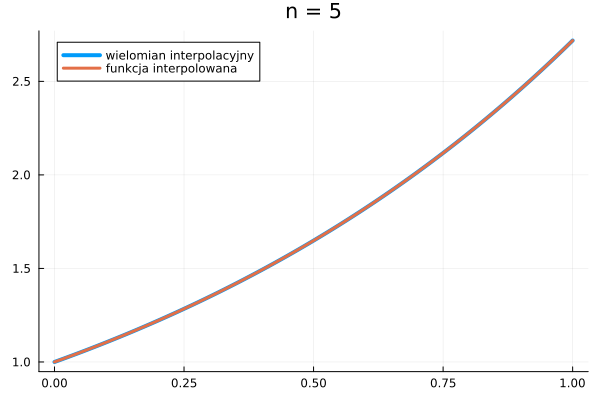
\includegraphics[scale=0.4]{5a_5.png}
\end{center}
\begin{center}
    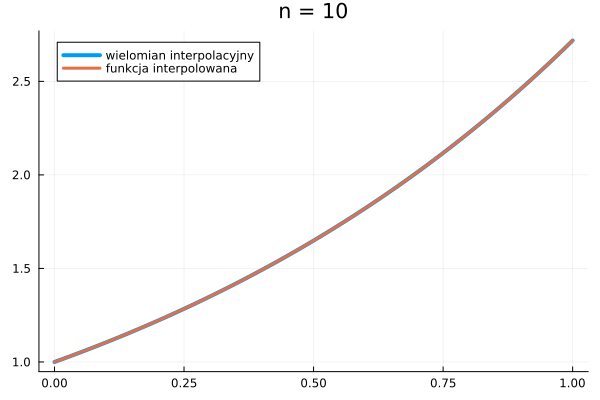
\includegraphics[scale=0.4]{5a_10.png}
\end{center}
\begin{center}
    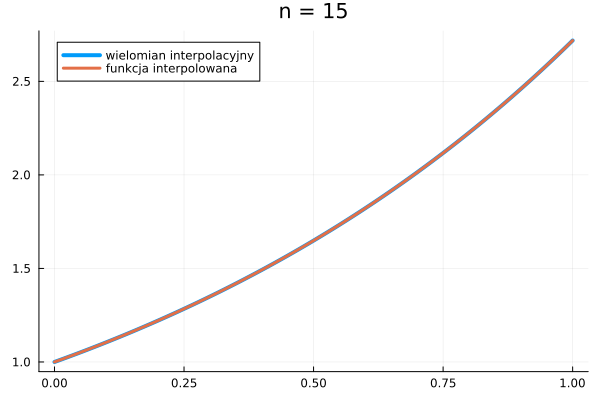
\includegraphics[scale=0.4]{5a_15.png}
\end{center}

\[
    x^2sin(x), [-1, 1], n = 5, 10, 15
\]

\begin{center}
    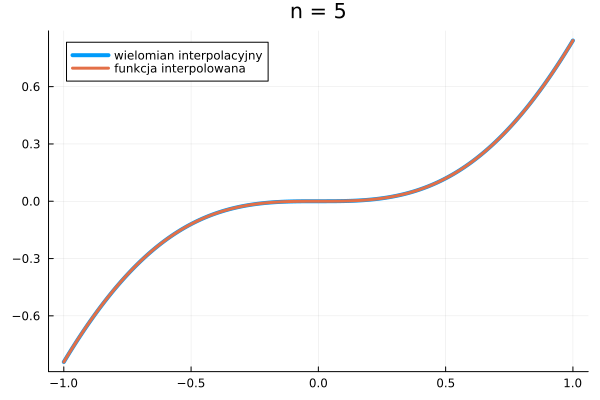
\includegraphics[scale=0.4]{5b_5.png}
\end{center}
\begin{center}
    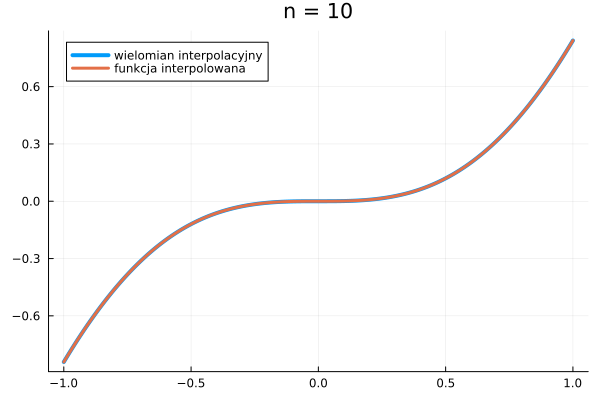
\includegraphics[scale=0.4]{5b_10.png}
\end{center}
\begin{center}
    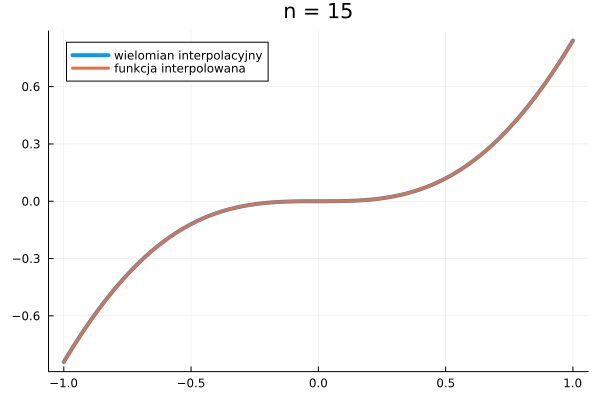
\includegraphics[scale=0.4]{5b_15.png}
\end{center}

\section*{Exercise 6}
\subsection*{Description of problem:}
In this exercise we are going to compare interpolating polynomials with interpolated functions for different numbers of n:


\subsection*{Results:}

\[
    |x|, [-1, 1], n = 5, 10, 15
\]

\begin{center}
    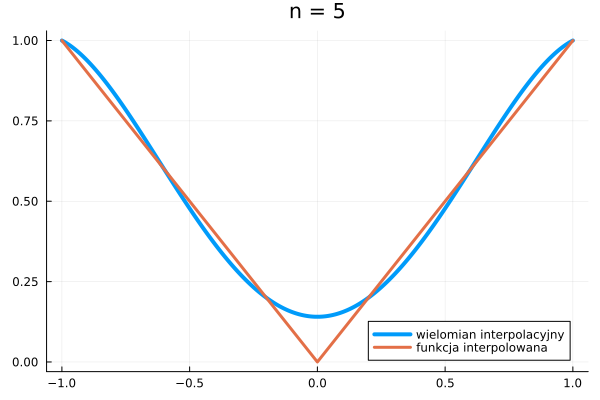
\includegraphics[scale=0.34]{6a_5.png}
\end{center}
\begin{center}
    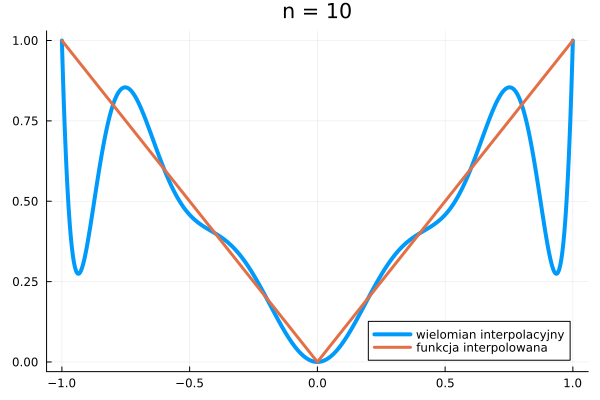
\includegraphics[scale=0.34]{6a_10.png}
\end{center}
\begin{center}
    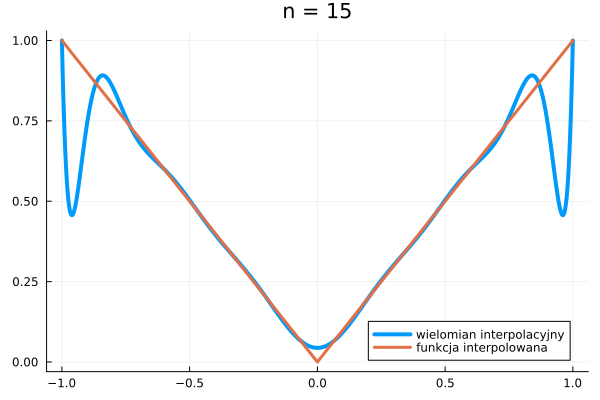
\includegraphics[scale=0.34]{6a_15.png}
\end{center}

\[
    \frac{1}{1 + x^2}, [-5, 5], n = 5, 10, 15
\]

\begin{center}
    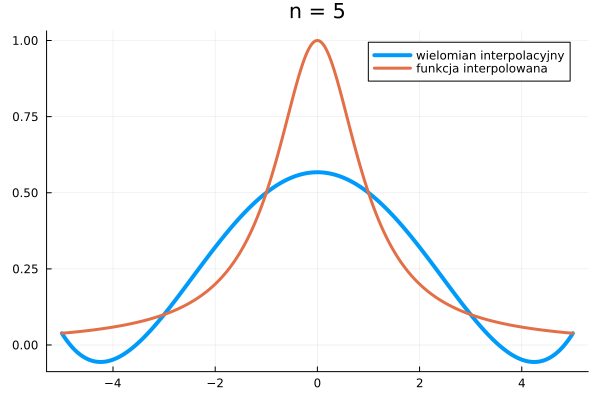
\includegraphics[scale=0.33]{6b_5.png}
\end{center}
\begin{center}
    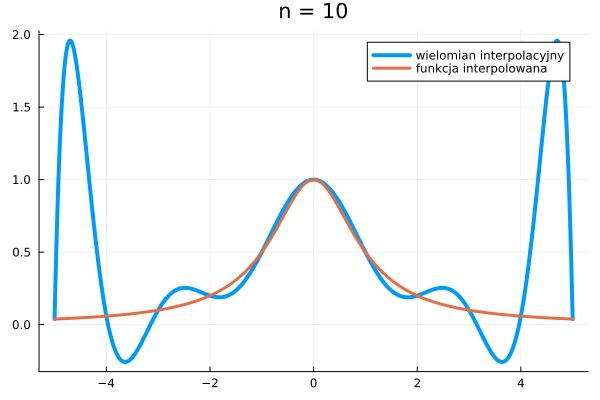
\includegraphics[scale=0.33]{6b_10.png}
\end{center}
\begin{center}
    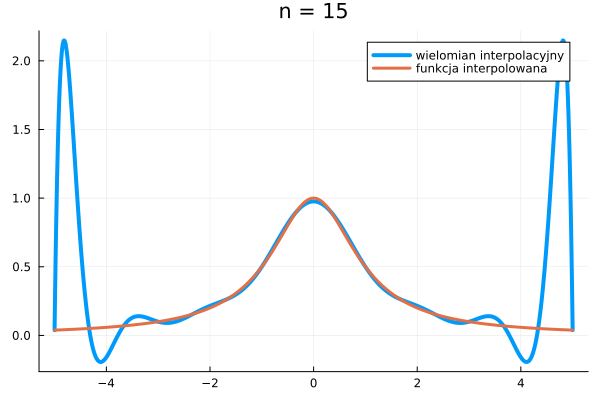
\includegraphics[scale=0.33]{6b_15.png}
\end{center}

\subsection*{Interpretation and conclusions:}
As we can see, for those functions, our approximation is not that good, especially near the edges of the range. What's more important is that the error will not go smaller with bigger n. A possible solution is to not take points evenly distributed, but instead take them from Chebyshev nodes, more nodes near the edges of the range, and less in the middle.

\end{document}